\documentclass[a0paper,portrait]{baposter}
\usepackage{tikz}

\bibliographystyle{ieeetr}  
\usepackage[toc,page]{appendix}
% we want ER + above/below + left/right
\usetikzlibrary{er,positioning}
\usepackage{tikz,mathpazo}
\usetikzlibrary{shapes.geometric, arrows}
\usepackage{pgfplots}
\usepackage{wrapfig}
\usepackage{lmodern}
\usepackage{tabu}
\usepackage[utf8]{inputenc} %unicode support
\usepackage[T1]{fontenc}
\usepackage{color}
\usepackage{tikz,mathpazo}
\usetikzlibrary{shapes.geometric, arrows}
\usepackage{flowchart}
\selectcolormodel{cmyk}
\usepackage[shortlabels]{enumitem} 
\setlist[enumerate]{nosep}
\graphicspath{{figures/}} % Directory in which figures are stored


\newcommand{\compresslist}{%
\setlength{\itemsep}{0pt}%
\setlength{\parskip}{1pt}%
\setlength{\parsep}{0pt}%
}

\newenvironment{boenumerate}
  {\begin{enumerate}\renewcommand\labelenumi{\textbf\theenumi.}}
  {\end{enumerate}}



\begin{document}


\definecolor{darkblue}{cmyk}{1,0.6,0,0.15}
\definecolor{lightblue}{cmyk}{1,0.6,0,0}
\definecolor{lightb}{cmyk}{0.3,0.15,0,0}

\begin{poster}
{
grid=false,
headerborder=open, % Adds a border around the header of content boxes
colspacing=1em, % Column spacing
bgColorOne=white, % Background color for the gradient on the left side of the poster
bgColorTwo=white, % Background color for the gradient on the right side of the poster
borderColor=darkblue, % Border color
headerColorOne=lightblue, % Background color for the header in the content boxes (left side)
headerColorTwo=lightblue, % Background color for the header in the content boxes (right side)
headerFontColor=white, % Text color for the header text in the content boxes
boxColorOne=white, % Background color of the content boxes
textborder=roundedsmall, %rectangle, % Format of the border around content boxes, can be: none, bars, coils, triangles, rectangle, rounded, roundedsmall, roundedright or faded
eyecatcher=false, % Set to false for ignoring the left logo in the title and move the title left
headerheight=0.11\textheight, % Height of the header
headershape=rounded, % Specify the rounded corner in the content box headers, can be: rectangle, small-rounded, roundedright, roundedleft or rounded
headershade=plain,
headerfont=\Large\textsf, % Large, bold and sans serif font in the headers of content boxes
%textfont={\setlength{\parindent}{1.5em}}, % Uncomment for paragraph indentation
linewidth=2pt % Wi dth of the border lines around content boxes
}
{}
%
%----------------------------------------------------------------------------------------
%	TITLE AND AUTHOR NAME
%-------------------------------------------------
{\sf\vspace{1em}
\title\textsf %Sans Serif
\color{blue}{\textbf{Realization of the Multi-\\ functional 
Robotic Vehicle}
}
} % Poster title
% {\vspace{1em} Marta Stepniewska, Pawel Siedlecki\\ % Author names
% {\small \vspace{0.7em} Department of Bioinformatics, Institute of Biochemistry and Biophysics, PAS, Warsaw, Pawinskiego 5a}} % Author email addresses
{\sf\vspace{0em}\\
\LARGE{\textsf{\qquad Student:\quad Shen Xiaofan \quad {\color{blue}\textbf{Thesis ID 80}}\\
\qquad Supervisor:  \\ \qquad Assessor:\quad  }}
\vspace{0.1em}\\
\small{  }
}
{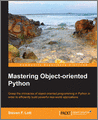
\includegraphics[width=0.53\linewidth]{logo}} % University/lab logo % Poster title
% {\vspace{1em} Marta Stepniewska, Pawel Siedlecki\\ % Author names
% {\small \vspace{0.7em} Department of Bioinformatics, Institute of Biochemistry and Biophysics, PAS, Warsaw, Pawinskiego 5a}} % Author email addresses
% University/lab logo

\headerbox{1. Abstract}{name=introduction,column=0,row=0, span=3}
{
\begin{wrapfigure}{l}{0.1\textwidth}
    \vspace{-15pt}
    \begin{center}
        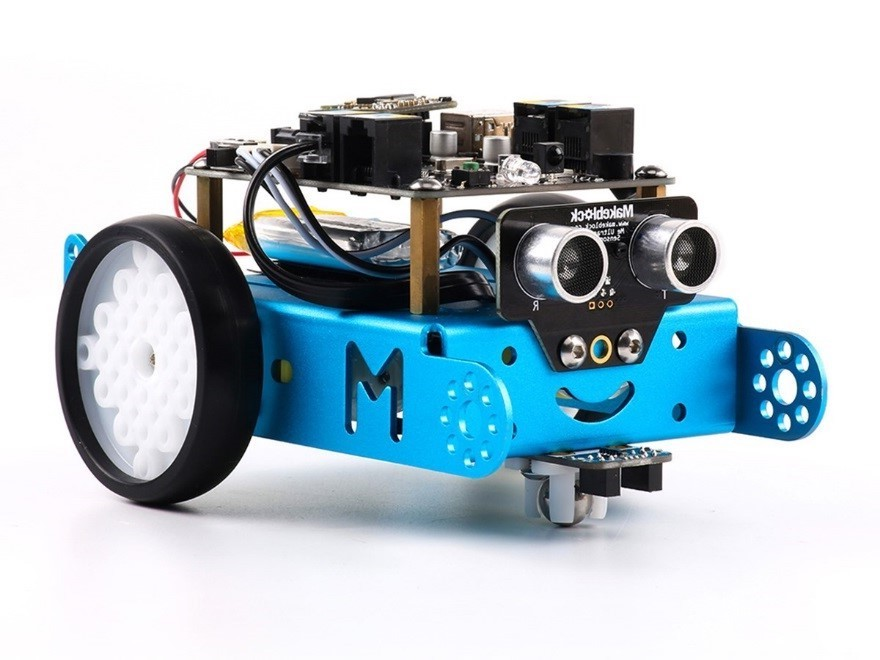
\includegraphics[width=\linewidth]{m2}
    \end{center}
    %\vspace{-145pt}
\end{wrapfigure}
\textsf 
{

Mesoscale eddy is an important research topic in the field of marine science. Among them, the detection of mesoscale vortices is an important research direction in mesoscale eddy research and has very important scientific significance. In recent years, deep neural networks in the field of artificial intelligence have developed rapidly, and they are widely used to solve many practical problems in computer vision. In this paper, the object detection algorithm in deep learning is applied to mesoscale eddy detection. Compared with the traditional mesoscale eddy detection method, only the position and size of the mesoscale eddy can be detected, which can better utilize multimodal information for positioning. Classification and instance segmentation. Based on the Mask-RCNN algorithm, this paper proposes an object detection algorithm combining multi-modal satellite remote sensing image data to identify, classify and segment mesoscale vortices in the ocean. The experimental results show that our method can effectively extract the features of mesoscale eddies and accurately detect and locate them. At the same time, our method obtains higher accuracy.

}

\headerbox{2. Introduction}{name=model,column=0,below=introduction,span=1}{
\textsf{Robotic prediction becomes a rapidly expanding field in recent years. Robot can achieve complex functions with sensors as hardware components are developed maturely, so the core part of this project is the software. The main aims are below: 
\begin{enumerate}[-]
\item Detect and calculate distance of an object;
\item Predict the distribution of obstacles;
\item Mapping the area of the surrounded space;
\end{enumerate}
\textbf{Ultrasonic sensor} is chosen for its lower price and simplicity to detect object and measure distance. \\
\textbf{Laser radar} is applied because buliding the grip map with radar is the best way to  detect the environment instantly and accurately. \\\textbf{SLAM} (Simultaneous Localization and Mapping) is selected as the method to estimate the robot pose and generate a map. } 
%\begin{center}
 %   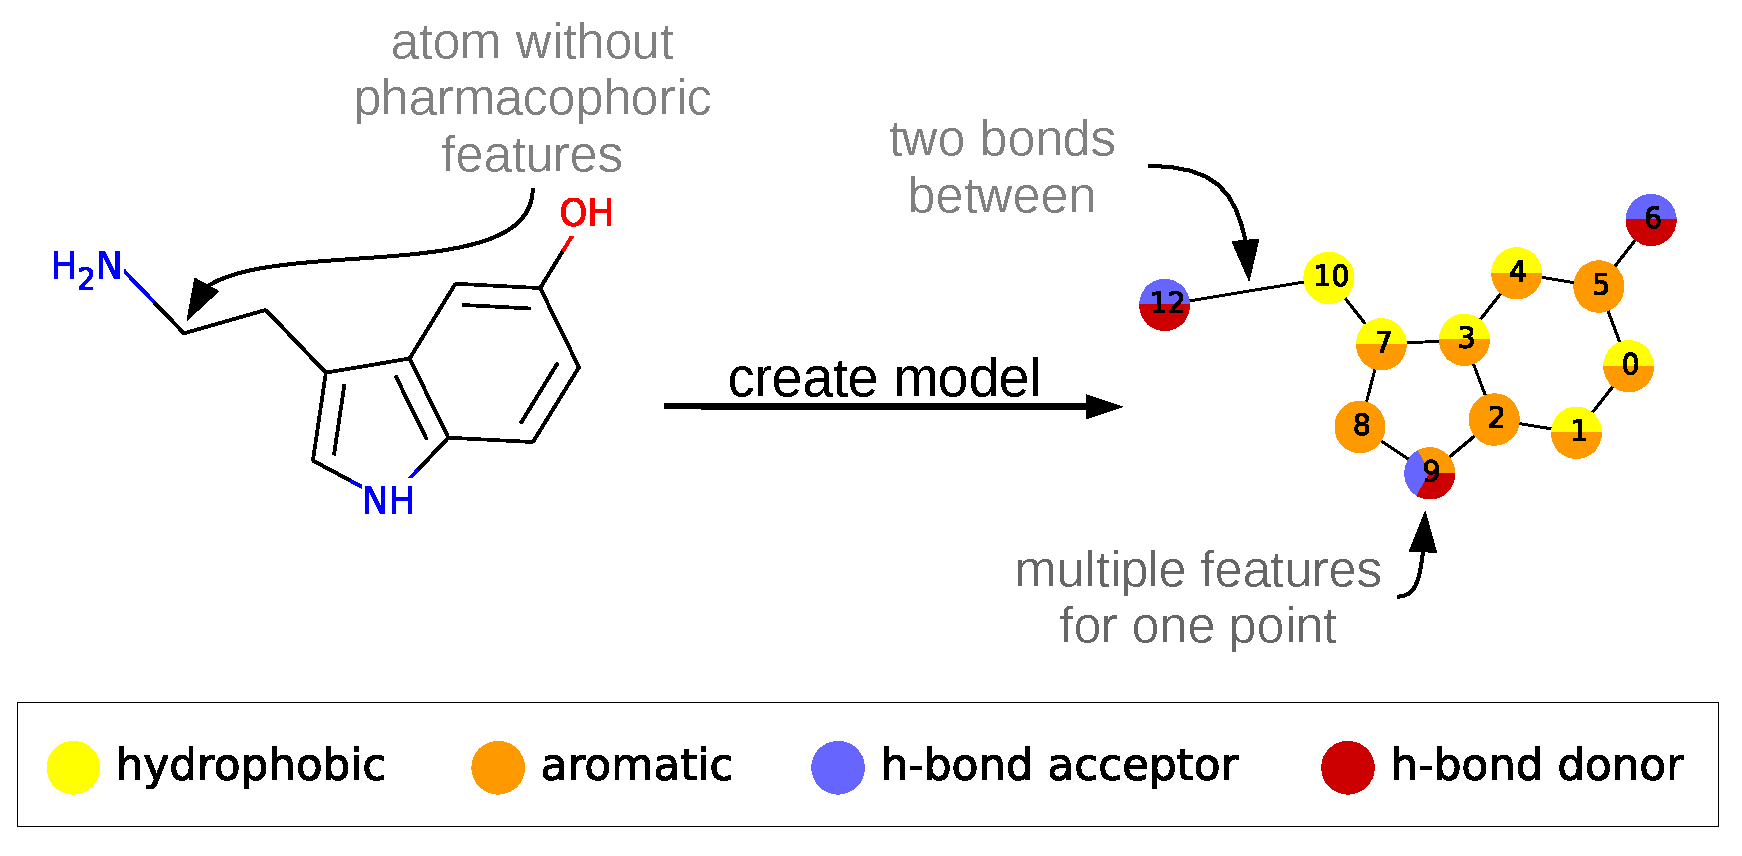
\includegraphics[width=\linewidth]{phar}
%\end{center}
%\vspace{-2pt}
}



\headerbox{3. Hardware and software design}{name=mcs,column=0,below=model,above=bottom,span=1}
{\textsf{{\color{blue}\textbf{Core part of hardware:\\}} mCore,Ultrasonic sensor.}\\
\includegraphics[width=1\linewidth]{list6}\\

\textsf{{\color{blue}\textbf{Core part of software:}}
\\
Flowchart of ultrasonic sensor }\cite{deng09study}
\\
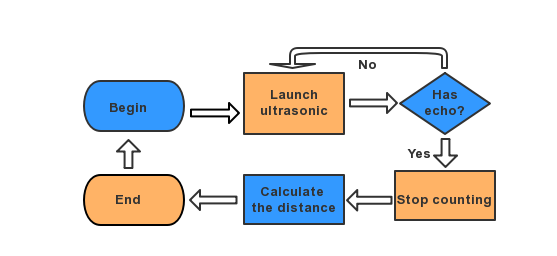
\includegraphics[width=1\linewidth]{yes}

\textsf{\textbf{Calculate the distance} means to calculate distance from sensor to obstacles by given formula; \\
\textbf{Has echo} means the reflection of ultrasonic.}\\

\textsf{{\color{blue}\textbf{Obstacle Avoidance Example in mblock:}}}
\center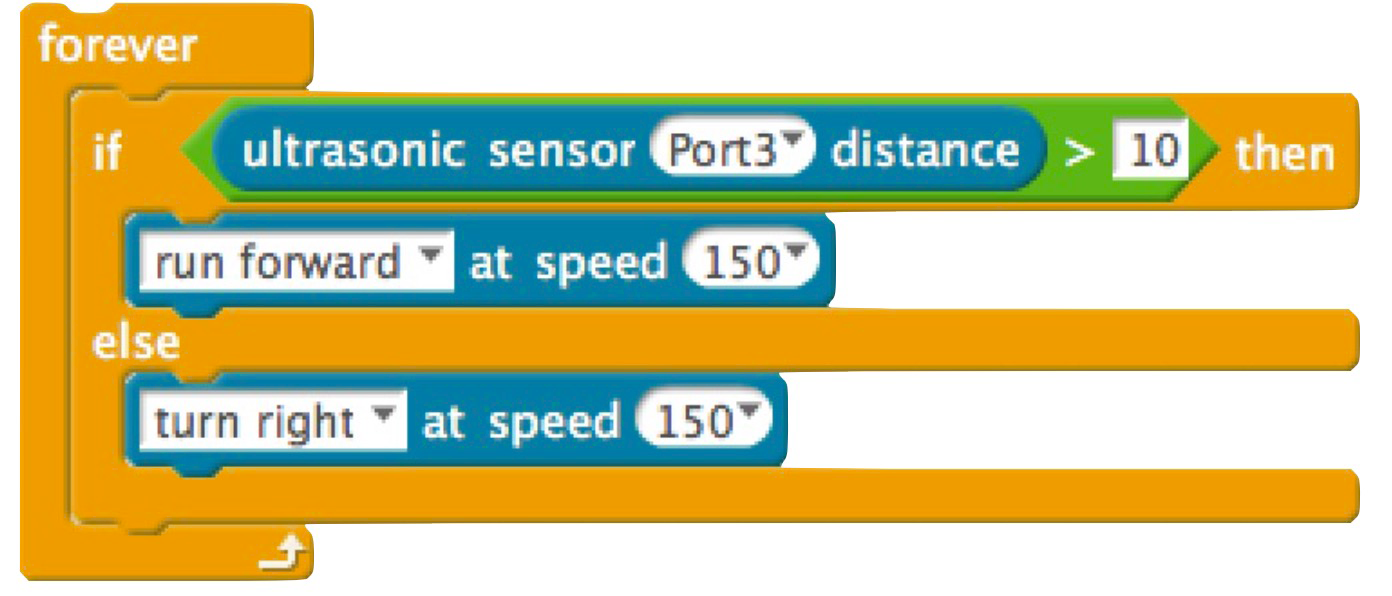
\includegraphics[width=0.95\linewidth]{lego3}

\textsf{\textbf{Explanation: }\\ Mblock contains a series of programming courses, which presents Arduino/C language iconically.\\ Below example: if the measured distance > 10cm, no obstacles are detected, robot runs forward, otherwise turns right and repeats the flow. }
}

\headerbox{4. Methodology}{name=screen,span=2,column=1,below=introduction}{ % To reduce this block to 1 column width, remove 'span=2'\textsl
{\color{blue}{\textsf{\textbf{\large{Ultrasonic Sensor: distance measurement}}}}}\\
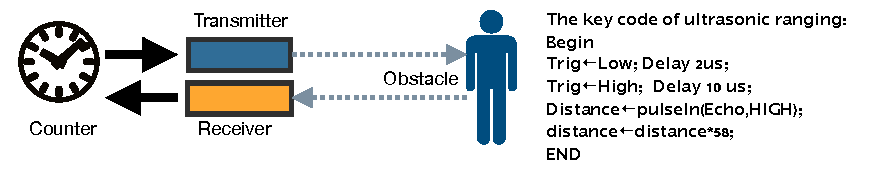
\includegraphics[width=1
\linewidth]{ops}
\textsf{\textbf{Ultrasonic} is launched when time starts,
 it runs into \textbf{obstacles} and reflect back to the \textbf{receiver end}, time counting stops right at this moment.  By applying the formula: \cite{song07design}
 \vspace{-1em}
 \begin{equation}
{\large\textsf{\textbf{$l=\frac{ct}{2}$}}}
\end{equation}
{ $l$ is distance from the robot,
$t$ is time from ultrasonic launched to the received,$c$ is the speed of ultrasonic.}}\\

{\color{blue}{\textsf{\textbf{SLAM flowchart (Simultaneous Localization and Mapping:)}}}}\\
\vspace{-4em}
\center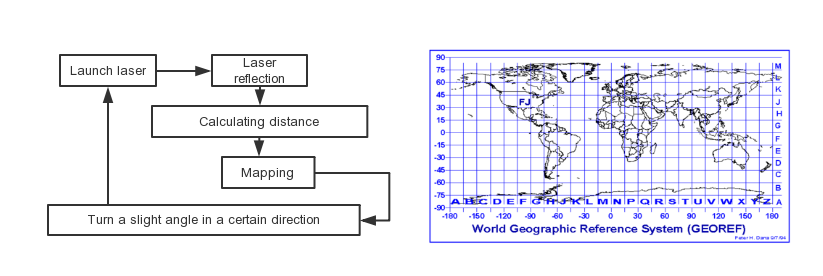
\includegraphics[width=1\linewidth]{map}
\vspace{-3em}
\begin{enumerate}[fullwidth,itemindent=-0.7em,label=(\arabic*)]
\item[] \textsf{\textbf{Grid mapping:}}
{\textsf{A grid can be analogized as a point in a coordinate system, above example is referred;\\ 1.Divide the whole environment into many grids in same size; 2.Drive the robot, get feedback information; 3.Predict the probability of existing  obtacles in every grids; 4.Give grayscale values to the evaluated grids. }}
\end{enumerate}
% We prepared datasets as shown in the left diagram.
% Then, we tested both classifiers 


}


\headerbox{5. Results And Analysis}{name=sea,span=2,column=1,below=screen}{ % To reduce this block to 1 column width, remove 'span=2'

\begin{wrapfigure}{r}{0.45\textwidth}
    \vspace{-22pt}
    \begin{center}\caption{\textsf{Error analysis:measured distance and actual distance are compared in this chart.}}
        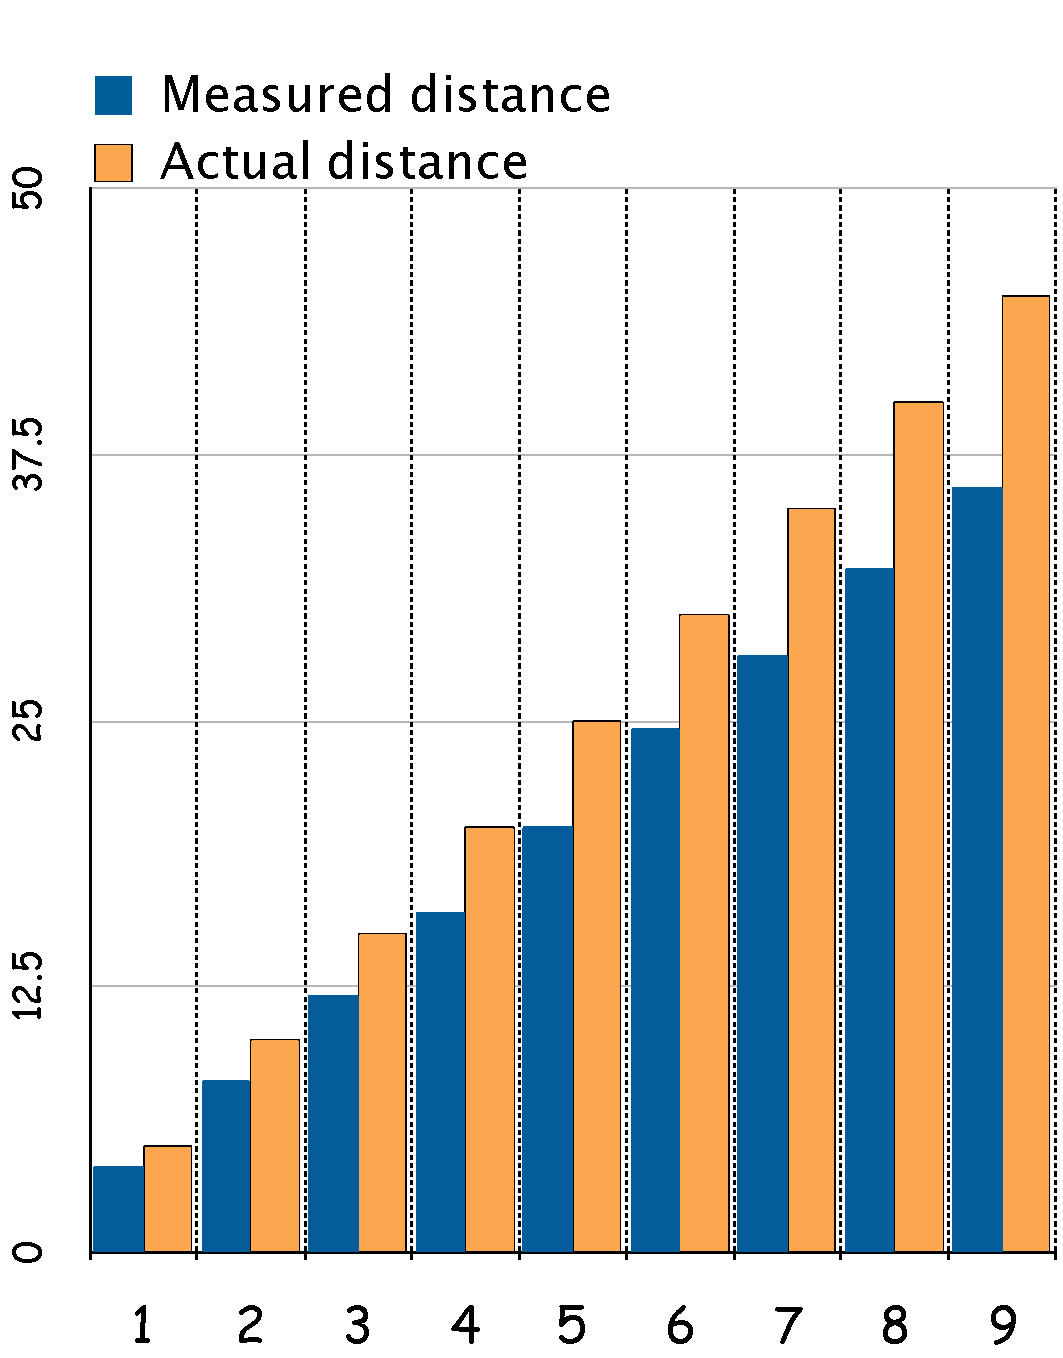
\includegraphics[width=0.71\linewidth]{chartff}
    \end{center}
    %\vspace{-145pt}
\end{wrapfigure}


% We tested DeCAF in 35 case studies taken from the DUD-E database, to evaluate its power to discriminate between active and inactive molecules.
% We used DeCAF as a classifier and compared it to the SEA (Similarity Ensemble Approach) algorithm \cite{keiser2007relating}.
% To compare sets of ligands, we adapted the approach used in SEA, replacing Tc by DCAF.
% We prepared datasets as shown in the left diagram.
% Then, we tested both classifiers calculating ROC AUC values for every target (below).
\textsf{\textbf{Real distance} and \textbf{measured distance} are recorded and compared based on the ultrasonic idstance measurement principle. The {\color{darkblue}tendency} is: more far the distance is, the error becomes bigger. \\ The relation between real and measured distance is:
\begin{equation}
{\textsf{\textbf{Y=1.25X}}}
\end{equation}
\vspace{-2pt} 
Where X is measured distance, Y is real distance. \\ Code should be modified to make the error minimum.
Real distance, measured distance and error (unit: cm):
}
% Please ask me about details.

\begin{tabular}{|c|c|c|c|}% 通过添加 | 来表示是否需要绘制竖线\textsl
\hline  % 在表格最上方绘制横线
\textsf{Number.} &\textsf{Real distance} &\textsf{Measured distance}&\textsf{$\Delta$error}\\
\hline  %在第一行和第二行之间绘制横线
1.&5.0&4.03& 0.97\\
\hline
2.&15.0&12.12&2.88\\
\hline
3.&25.0&20.01&4.99\\
\hline
4.&35.0&28.00&7.00\\
\hline
5.&45.0&36.01&3.99\\
\hline % 在表格最下方绘制横线
\end{tabular}

}


\headerbox{6. Conclusions And Future Work}{name=conclusion,column=1,below=sea,span=2}{
\textsf{Distance measurement is completed and improved by finding out the relationship between actual distance and measured distance. Simulation shows that error is minimized by programming output distance based on the original one, afterwards object avoidance is accomplished. Object prediction will be tested again by radar, as radar collects more data compared with ultrasonic sensor, which will contribute to the core: mapping. SLAM has been used in cleaning robot, in future, such robots can be applied in unexpected and dangerous environment, where human beings are not available, to detect, predict and explore. }}

\headerbox{7.Selected References}{name=ref,column=1,span=2,below=conclusion,above=bottom}{


%\small % Reduce the font size in this block
\renewcommand{\section}[2]{\vskip 0.05em} % Get rid of the default "References" section title
%\nocite{*} % Insert publications even if they are not cited in the poster

\begin{thebibliography}{x}
\vspace{-0.5em}
\bibitem{deng09study} \textsf{L. Deng, Study on Ultrasonic Ranging System Design,Aug. 2009}
\vspace{-1em}
\bibitem{song07design} \textsf{K.Song Y.C.Chen and J.C.Zhao "The Design of Ultrasonic Ranging Sensor with Dual Output Functions" Control  amp; Automation vol. 23 pp.168-170,  Dec. 2007.} 
\end{thebibliography}


}
\end{poster}

\end{document}
